%%%%%%%%%%%%%%%%%%%%%%%%%%%%%%%%%%%%%%%%%%%%%%%%%%%%%%%%%%%%%%%%%%
% Sample template for MIT Junior Lab Student Written Summaries
% Available from http://web.mit.edu/8.13/www/Samplepaper/sample-paper.tex
%
% Last Updated April 12, 2007
%
% Adapted from the American Physical Societies REVTeK-4 Pages
% at http://publish.aps.org
%
% ADVICE TO STUDENTS: Each time you write a paper, start with this
%    template and save under a new filename.  If convenient, don't
%    erase unneeded lines, just comment them out.  Often, they
%    will be useful containers for information.
%
% Using pdflatex, images must be either PNG, GIF, JPEG or PDF.
%     Turn eps to pdf using epstopdf.
%%%%%%%%%%%%%%%%%%%%%%%%%%%%%%%%%%%%%%%%%%%%%%%%%%%%%%%%%%%%%%%%%%


%%%%%%%%%%%%%%%%%%%%%%%%%%%%%%%%%%%%%%%%%%%%%%%%%%%%%%%%%%%%%%%%%%
% PREAMBLE
% The preamble of a LaTeX document is the set of commands that precede
% the \begin{document} line.  It contains a \documentclass line
% to load the REVTeK-4 macro definitions and various \usepackage
% lines to load other macro packages.
%
% ADVICE TO STUDENTS: This preamble contains a suggested set of
%     class options to generate a ``Junior Lab'' look and feel that
%     facilitate quick review and feedback from one's peers, TA's
%     and section instructors.  Don't make substantial changes without
%     first consulting your section instructor.
%%%%%%%%%%%%%%%%%%%%%%%%%%%%%%%%%%%%%%%%%%%%%%%%%%%%%%%%%%%%%%%%%%

\documentclass[aps,twocolumn,secnumarabic,balancelastpage,amsmath,amssymb,nofootinbib]{revtex4}

% Documentclass Options
    % aps, prl stand for American Physical Society and Physical Review Letters respectively
    % twocolumn permits two columns, of course
    % nobalancelastpage doesn't attempt to equalize the lengths of the two columns on the last page
        % as might be desired in a journal where articles follow one another closely
    % amsmath and amssymb are necessary for the subequations environment among others
    % secnumarabic identifies sections by number to aid electronic review and commentary.
    % nofootinbib forces footnotes to occur on the page where they are first referenced
        % and not in the bibliography
    % REVTeX 4 is a set of macro packages designed to be used with LaTeX 2e.
        % REVTeX is well-suited for preparing manuscripts for submission to APS journals.


\usepackage{lgrind}        % convert program listings to a form includable in a LaTeX document
\usepackage{chapterbib}    % allows a bibliography for each chapter (each labguide has it's own)
\usepackage{color}         % produces boxes or entire pages with colored backgrounds
\usepackage{graphics}      % standard graphics specifications
\usepackage[pdftex]{graphicx}      % alternative graphics specifications
\usepackage{longtable}     % helps with long table options
\usepackage{epsf}          % old package handles encapsulated post script issues
\usepackage{bm}            % special 'bold-math' package
\usepackage{asymptote}     % For typesetting of mathematical illustrations
\usepackage{thumbpdf}
\usepackage[colorlinks=true]{hyperref}  % this package should be added after all others
                                        % use as follows: \url{http://www.usm.maine.edu/~pauln/MainSite/PHY240.html}


%
% And now, begin the document...
% Students should not have to alter anything above this line
%

\begin{document}
\title{Bessel's Corrections to the Keter Pendulum \\ 
\textit{Determining Gravitation Acceleration on Earth}}
\author         {A. Knight, N. Anna}
\email          {alexander.knighr@maine.edu, nicholas.anna@maine.edu}
%\homepage{http://www.usm.maine.edu/~pauln/phy240/}
\date{\today}
\affiliation{USM Department of Physics}


\begin{abstract}
We attempted to experimentally determine the standard gravitational acceleration $g$ by means of a Bessel pendulum, which is a volume symmetric, mass asymmetric reversible pendulum that can be treated as a simple pendulum without consideration to the moment of inertia or most air resistance when the period of each orientation is equivalent. Our experiment consisted of changing the center of mass of the pendulum to equalize the periods. From this period, we then calculated $g=(9.781 \pm 0.017) \frac{m}{s^2}$, which gave us an experimental error of $0.262\%$. Despite a small experimental error, our uncertainty failed to encompass the actual value of $g=9.80665 \frac{m}{s^2}$.

\end{abstract}

\maketitle

%%%%%%%%%%%%%%%%%%%%%%%%%%%%%%%%%%%%%%%%%%%%%%%%%%%%%%%%%%%%%%%%%%

%An important part of your education as a physicist is learning to
%use standard tools which enable you to share your work with others.
%In iLab, we will instruct you in the use of \LaTeX on either
%the laboratory's Mac or Linux machines  or your own personal computer to
%write scientific papers in a widely accepted professional style. The
%source file
%\footnote{\url{web.mit.edu/8.13/www/Samplepaper/sample-paper.tex}}
%for this document may be used as a template for your Junior Lab
%papers. Spending a few hours studying and altering this document
%will allow you to develop sufficient mastery of \LaTeX to easily
%generate all manner of technical documents.  Specific instructions
%for compiling \LaTeX documents on Windows and Athena systems are
%contained in the Appendices.  The Writing
%Process\footnote{\url{web.mit.edu/writing/Resources/Writers/process.html}}
%involves at least four distinct steps: prewriting, drafting,
%revising and editing.  Given the tight time constraints in 
%iLab, students are advised to begin the drafting process {\bf before}
%finishing their lab sessions.  While final results and analysis are
%not possible, much of the draft can be accomplished during the
%latter sessions of an experiment.
%
%The written report introduction should succinctly report the
%motivation, purpose and relevant background to the experiment.
%%%%%%%%%%%%%%%%%%%%%%%%%%%%%%%%%%%%%%%%%%%%%%%%%%%%%%%%%%%%%%%%%%%%%%%%%%%%%
% This is a basic figure drawn using the asymptote package
% see http://asymptote.sourceforge.net/ for more information
%\begin{figure}
%\centering
%\begin{asy}
%size(3cm);
%draw(unitcircle);
%\end{asy}
%\caption{Embedded Asymptote Figure} \label {fig:asymptote1}
%\end{figure}
%%%%%%%%%%%%%%%%%%%%%%%%%%%%%%%%%%%%%%%%%%%%%%%%%%%%%%%%%%%%%%%%%%%%%%%%%%%%%%
%\subsection{Expository Writing}
% The essence of expository writing is the communication of understanding
%through a clear and concise presentation of predominately factual
%material.\cite{mayfield1998,pritchard1990} Most people cannot
%compose successful expository prose unless they put the need to
%communicate foremost among their priorities. Two things predominate
%in generating understanding in the reader:
%\begin{enumerate}
%\item ORGANIZATION: The reader must be provided with an overview or
%outline, know how each fact that he reads fits into that overall
%picture, and he must be alerted if it is an especially important
%fact. Furthermore, the facts must be presented in a logical order
%(so that fact 17 is not important for understanding fact 12).
%
%\item UNIFORM DEPTH of PRESENTATION: Bearing in mind the preexisting
%knowledge of the reader, the writer must budget the length of
%discussion allotted to each topic in proportion to its importance.
%
%\end{enumerate}
%
%Of course clarity of presentation and elegance of explanation will
%greatly enhance the ease and pleasure of understanding; still, a
%murky explanation can be fairly useful if the reader has been told
%what he is reading about and where it fits into the overall scheme
%of things - especially if the reader is familiar with the general
%subject matter under discussion.
%
%The Junior lab writeup is one of the few opportunities
%undergraduates are given to practice technical writing. Thus we urge
%you to concentrate on your overall presentation, not only on the
%facts themselves. We strongly recommend that you:
%\begin{enumerate}
%\item Base your report on an outline.
%\item Begin each paragraph with a topic sentence which expresses the
%main area of concern and the main conclusion of the paragraph. Put
%less important material later in the paragraph.
%\end{enumerate}
%
%Point 2 is frequently absent in 8.13 reports; they are your
%mechanism for telling the reader what the topic under discussion is
%and where it fits into the overall picture.
%
%You can check your topic sentences by reading them in order (i.e.
%omit all the following sentences in each paragraph) - this should
%give a fair synopsis of your paper.
%
%If you are individually writing up results you obtained with a
%partner, use we and I appropriately.
%
%Use the past tense for your procedure and analysis, the past perfect
%for preparation and the present for emphasis or conclusions, e.g.
%``Since we had previously measured constructive and destructive
%interference, we concluded that electrons are waves.''
%
%\begin{enumerate}
%\item Be sure your Figures have comprehensible captions.
%
%\item Make a complete estimate of your errors (not just statistical) - even
%if it's crude.
%
%\item Trace origin of formulae you use (e.g. Moseley's Law) to well known
%physics (in this case to the Bohr atom) - don't derive, just
%indicate what new assumptions are needed.
%\end{enumerate}
%
%Please consult the MIT's Online Writing and Communications Center's
%web page\footnote{MIT Online Writing and Communication Office:
%\url{web.mit.edu/writing/}} for further guidance in all aspects of
%writing, style and to make appointments with consultants for free
%advice.  They even have an on-line tutor to which you can submit
%sections of your paper for critique at any stage of the writing
%process!!!
%
%{\bf Lastly: Remember to proofread your paper for spelling and grammar
% mistakes.  Few things are as offensive to a reviewer as careless
% writing and such mistakes will count against you!}
%
\section{Problem and Relevant Theory}

Pendulums are a prominent tool in classical and modern physics. The oscillatory motion of the pendulum is well known and easily modeled with mathematics. They can be manufactured in order to customize and emphasize many aspects of the pendulum itself.
 
Pendulums were often used to measure the gravitational force due to their sensitivity and gravity's weak attraction. Today, we have more modern methods using lasers and vacuum chambers, but the old methods are still important and informative.

In 1817 Henry Kater designed and tested a reversible pendulum that was meant to measure the gravitational acceleration of the Earth. From this, Kater showed that the center of gravity and moment of inertia did not have to be calculated. By adjusting small weights on the pendulum, he would change the center of mass, and so change its period. He could then adjust the pendulum until the period was the same for both pivot points. From here, it could be treated as a simple pendulum, where $T^2 = 4\pi^2\dfrac{l}{g}$. This method was mostly effective, but it failed to take into account several factors that changed the period between the two pivot points, such as air resistance, buoyancy, and the added mass of the air dragged behind. 

These problems reduced the accuracy of the reversible pendulum until in 1826 Friedrich Bessel designed a pendulum that was symmetric in volume, but asymmetric in mass. This negated the need to determine most air resistance. Additionally, by balancing the pendulum on a knife blade to find the center of mass, he then could determine the pendulum's period. This design was used for years to make fine measurements of the acceleration of gravity.

%
%The report should be type-written in a form that would be suitable
%for submission as a manuscript for publication in a professional
%journal such as Physical Review Letters\footnote{Physical Review
%Letters: \url{prl.aps.org/}}. One helpful resource is the APS
%Physics Review Style and Notation Guide\footnote{ APS Physics Style
%and Notation Guide: \url{publish.aps.org/STYLE/}}. Figures (created
%as PDF files) should be inserted into the text in their natural
%positions. The body of the summary should include a discussion of
%the theoretical issues addressed by the experiment. This should be
%done at a level, so that another 8.13 student could follow your
%development.
%
%\subsection{Typesetting Mathematics}
%
%One of the great powers of \LaTeX is it's ability to typeset all
%manner of mathematical expressions.  While it does take a short
%while to get used to the syntax, it will soon become second nature.
%Numbered, single-line equations are the most common type of equation
%in \textit{Junior Lab papers} and are usually referenced in the
%text; e.g. see Equation~(\ref{eq:first-equation}).
%%
%\begin{equation}
%   \chi_+(p)\alt{\bf [}2|{\bf p}|(|{\bf p}|+p_z){\bf ]}^{-1/2}
%   \left(
%   \begin{array}{c}
%      |{\bf p}|+p_z\\
%      px+ip_y
%   \end{array}\right)
%\,. \label{eq:first-equation}
%\end{equation}
%%
%% Be sure there is NO EMPTY LINE after \end{quation} and before the
%% following lines, if you do not want a new paragraph to start there
%% (and be indented).
%%
%Mathematics can also be placed directly in the text using
%delimeters: $\vec{\psi_1} = |\psi_1\rangle \equiv c_0|0\rangle +
%c_1|1\rangle \chi^2 \approx
%\prod\sum\left[\frac{y_i-f(x_i)}{\sigma_i}\right]^2 |\psi_1\rangle
%\sim \lim_{\mu \rightarrow \infty}p(x;\mu) \geq \frac{1}{\sqrt{2 \pi
%\mu}} e^{-(x-\mu)^2 / 2\mu}P(x) \ll \int_{-\infty}^x p(x')dx'a
%\times b \pm c \Rightarrow \nabla \hbar$.
%
%Infrequently, you may wish to typeset long equations which span more
%than one line of a two-column page.  A good solution is to split-up
%the equation into multiple lines and label all with a single
%equation number, like in Equation~\ref{eq:multilineeq}.  See the
%\LaTeX file to see how this is done.
%%
%\begin{eqnarray}
%  \sum \vert M^{\text{viol}}_g \vert ^2 
%   &=&  g^{2n-4}_S(Q^2)~N^{n-2} (N^2-1)
%\nonumber
%\\
%   &&   \times \left( \sum_{i<j}\right) \sum_{\text{perm}}
%            \frac{1}{S_{12}}  \frac{1}{S_{12}} \sum_\tau c^f_\tau
%\,.
%\label{eq:multilineeq}
%\end{eqnarray}
%
%Finally, it is often useful to group related equations to denote their
%relationship, e.g. in a derivation.  Enclosing single-line and
%multiline equations in \verb+\begin{subequations}+ and
%\verb+\end{subequations}+ will produce a set of equations that are
%``numbered'' with letters, as shown in Equations.~(\ref{subeq:1}) and
%(\ref{subeq:2}) below:
%\begin{subequations}
%\label{eq:whole}
%\begin{equation}
%  \left\{
%      abc123456abcdef\alpha\beta\gamma\delta1234556\alpha\beta
%       \frac{1\sum^{a}_{b}}{A^2}
%  \right\}
%%
%\,\label{subeq:1}
%\end{equation}
%\begin{eqnarray}
%  {\cal M} &=& ig_Z^2(4E_1E_2)^{1/2}(l_i^2)^{-1}
%                (g_{\sigma_2}^e)^2\chi_{-\sigma_2}(p_2)
%\nonumber\\
%  &&\times [\epsilon_i]_{\sigma_1}\chi_{\sigma_1}(p_1).\label{subeq:2}
%\end{eqnarray}
%\end{subequations}
%
%
%%%%%%%%%%%%%%%%%%%%%%%%%%%%%%%%%%%%%%%%%%%%%%%%%%%%%%%%%%%%%%%%%%%%%%%%%%%%%%
\section{Experimental Sketch and Salient Details}
Kater's pendulum design uses the symmetrical behavior of the period around the center of mass of an object. Following the logic and thought of Candela\cite{Candela2001}, we start with the equation for small oscillations of a physical pendulum,
\begin{equation}
\omega^2 = \dfrac{gml}{I}
\end{equation}
where $\omega$ is the angular frequency, $m$ is the mass of the pendulum, $l$ is the length, and $I$ is the moment of inertia. Draw a line through your center of mass, and pick an arbitrary origin such that $x_{cm} \geq 0$, then let your pendulum pivot at any point on this line $(x)$. By the Parallel axis theorem, our equation of motion is
\begin{equation}
\dfrac{\omega^2}{g} = \dfrac{m(x-x_{cm})}{I_{cm} +m(x-x_{cm})^2} 
\end{equation}
From here, we can solve for the effective length of our pendulum ($x-x_{cm}$), which gives us a quadratic equation that yields
\begin{equation}
x-x_{cm} = \pm \dfrac 1{2F} \pm \sqrt{\dfrac 1{4F^2} - \dfrac {I_o} {m}} 
\end{equation}
where $F = \dfrac {m(x-x_{cm})}{(I_o + m(x-x_cm)^2)}$. This equation defines four points symmetric around the center of mass at which the angular frequency is equal. By choosing two points such that they are asymmetric and opposite around the center of mass, the radical drops out of the equation, and the moment of inertia does not have to be taken into account. This then give 
\begin{equation}
\Delta x = \dfrac g{\omega_o^2}
\label{Eq:eq1}
\end{equation}
 which is expected for a simple pendulum.

\begin{figure}
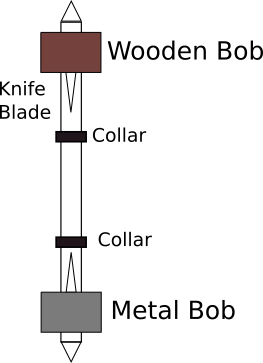
\includegraphics[scale=0.5]{pendulumDiagram.png}
\caption{Bessel Pendulum Diagram: Our pendulum consisted of three main parts. On either end of a solid metal were two bobs of equal volume and shape, one of wood and the other of brass, shown in brown and gray. Two sets of knife blades extended from the bobs to act as pivot points for the far side. Two movable collars are mounted between the knife blades, allowing for adjustments to the center of mass. This design allowed us to change the center of mass of the pendulum while keeping it symmetric.}
\label{fig:Diagram}
\end{figure}

Our apparatus (Fig \ref{fig:Diagram}) consists of a pair of symmetrical bobs about a meter apart on a metal pole, one wood and the other brass. Mounted below each bob is a knife edge that rests on a glass plate that the far bob uses as a pivot point. Two collars between the knife blades can be moved to change the center of mass. The pendulum is volume symmetric about the center line, but it is mass asymmetric due to the different densities of the bobs. 

To determine the center of mass for which the period is equal for both ends of the pendulum, the collars were moved symmetrically away from the knife edge in set increments, and the period was measured. Plotting the period versus the collar distance from the blades gave a linear relationship, with each bob having a different slope and intercept. By comparing where these lines crossed, we could then find the position of the collars that would result in an equal period. We then used equation \ref{Eq:eq1} to find $g$.

The period of the pendulum was measured by means of a photogate. As the pendulum oscillated the bottom tip broke the infrared beam from the photogate, and a timestamp was recorded. By analyzing the timestamps, a period was determined.


%
%This section describes the main components of the apparatus,
%procedures used and always makes reference to a figure(s) which
%contains a block diagram or schematic of the apparatus and perhaps
%includes the most important signal processing steps. {\bf The figure
%should be referenced as early as possible in this section with the
%placement of the figure as close to the descriptive text as is
%possible.}  It is usually necessary to place additional information
%within the figures themselves or in their captions for which there is
%no room in the main body of text.  This will help you stay within the
%two page limit.
%
%{\bf Example first sentence of an experimental section}
%The experimental apparatus consists of a specially prepared chemical
%sample containing $^{13}$CHCl$_3$, a NMR spectrometer, and a control
%computer, as shown in Figure~\ref{fig:samplefig}.
%
%%
%% Note, when including figures in a TeX document,
%% we suggest you first create the figures as
%% PDF files and then include them in the following way -
%% without the .pdf suffix)
%%
%
%\begin{figure}[htb]
%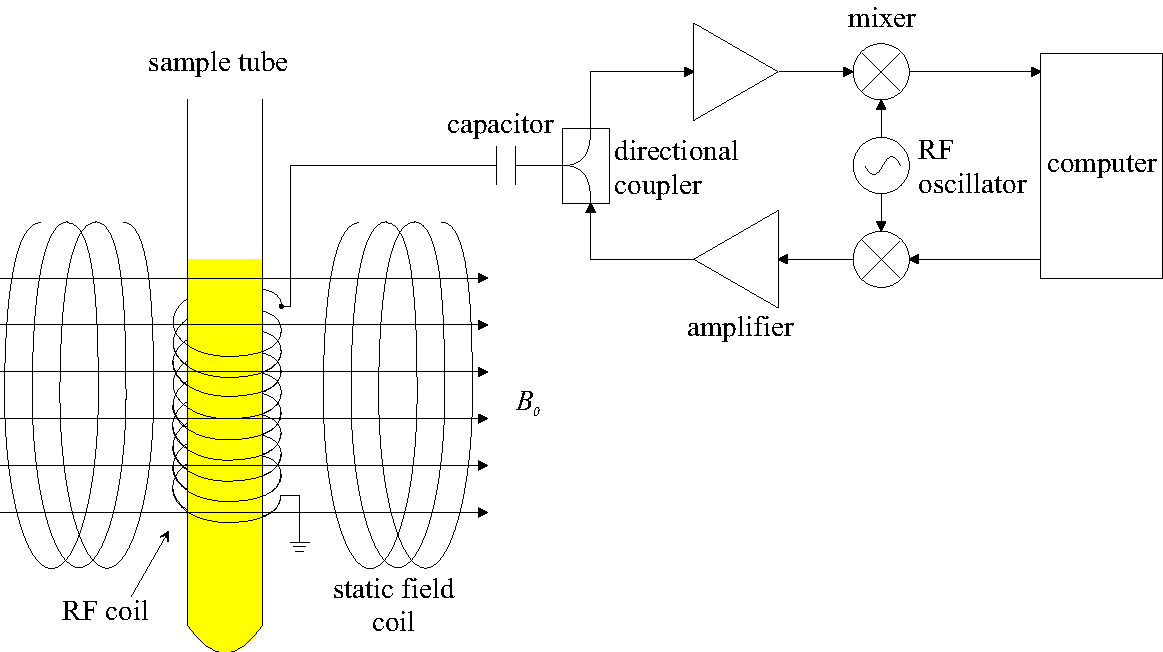
\includegraphics[width=8cm]{sample-fig1}
%\caption{This is a schematic of the main apparatus.  Use the caption
%space to elaborate on specific issues or complication, or operating
%procedures.  Especially valuable given the limited about of space in
%the main body of text.  The size of this graphic was set by the width
%command, the aspect ratio defaults to 1.0 if the height is not also
%set. Adapted from \cite{melissinos1966,melissinos2003}.\label{fig:samplefig}}
%\end{figure}
%
%
%
%%%%%%%%%%%%%%%%%%%%%%%%%%%%%%%%%%%%%%%%%%%%%%%%%%%%%%%%%%%%%%%%%%%%%%%%%%%%%%
\section{Data Presentation and Error Analysis}

The initial data collection was to determine roughly the point at which the two periods were equal, so that we could then take finer data in the region of interest.

\begin{figure}
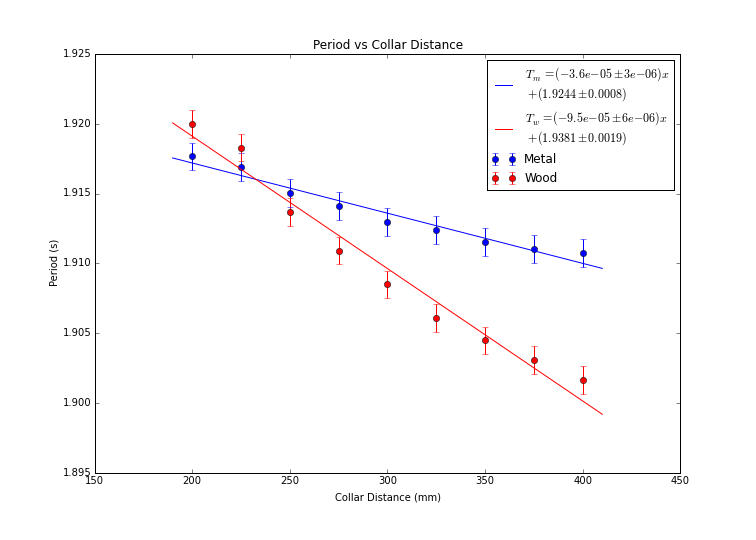
\includegraphics[width=\linewidth]{periodVsCollar.png}
\caption{Period versus collar distance: The collars on our pendulum were moved in set increments and the period of each side was taken. The point where the two lines cross show the approximate location at which the periods should be equal, and the difference in air resistance is negligible. We found this value to be around $232.7mm$.}
\label{fig:PvC}
\end{figure}

The collars were initially set $200mm$ away from the blades, and moved inward in $25mm$ increments, until the collars could not be moved closer together. This gave us the graph shown in figure \ref{fig:PvC}. From this graph we could see that our area of interest was approximately at $230mm$. Algebraic calculation of the interception point of the lines gave $232.66mm$.

We then took finer date, from $229mm$ to $231mm$. We stopped taking data after $231mm$ because we noticed that the difference between the period was increasing. We got the following table:
\begin{center}
\begin{tabular}{||c||c|c|c||c|c|c||}
\hline 
$\Delta X(mm)$ & Metal $T$ & Wood $T$ & $\Delta T$ & Metal $\omega$ & Wood $\omega$ & $\Delta \omega$ \\
\hline
229.0	& 1.91500	&	1.91717	&	0.0022	&	3.281	&	3.277	&	0.004\\
\hline
229.5	& 1.91695	&	1.91757	&	0.0006	&	3.278	&	3.277	&	0.001\\
\hline
230.0	& 1.91666	&	1.91759	&	0.0009	&	3.378	&	3.277	&	0.002\\
\hline
230.5	& 1.91629	&	1.91699	&	0.0007	&	3.279	&	3.278	&	0.001\\
230.5	& 1.91748	&	1.91713	&	0.0003	&	3.277	&	3.277	&	0.001\\
230.5	& 1.91626	&	1.91754	&	0.0013	&	3.279	&	3.277	&	0.002\\
230.5	& 1.91687	&	1.91797	&	0.0011	&	3.278	&	3.276	&	0.002\\
230.5	& 1.91631	&	1.91736	&	0.0010	&	3.279	&	3.277	&	0.002\\
\hline
231.0	& 1.90721	&	1.91820	&	0.0110	&	3.294	&	3.276	&	0.019\\
\hline
\end{tabular}
\label{tab:FineData}
\end{center}
Here, $\Delta X$ is the separation from the blades to closest side of the collars, $T$ is the period of the pendulums in seconds, and $\omega$ is the angular frequency. The five measurements at $230.5mm$ was to determine the uncertainty in our period measurements. 

We determined the equal period for each side of the pendulum ($T_o$) to be $1.917s \pm 0.001s$. From this we calculate the angular frequency to be $\omega_o = 3.277 \frac{rad}{s} \pm 0.002 \frac{rad}{s}$.

We measured the distance between the two pivot points to be $910.887mm \pm 0.5mm$. This relatively large error was due to the difficulty in keeping our measuring device lined up with the pendulum. If it became askew, it would add as much as a millimeter, despite being much more precise. 

From here, we can determine $g$:
\begin{align}
g&=(\Delta x) (\omega_o)^2\\
g&=(0.910887m \pm 0.0005m)(3.277 \frac{rad}{s} \pm 0.002 \frac{rad}{s})^2 \\
g&=9.781 \frac{m}{s^2} \pm 0.017 \frac{m}{s^2}
\end{align}

The maximum value inside our uncertainty, $9.798 \frac{m}{s^2}$ just comes under the accepted value for $g$, which is $9.80665 \frac{m}{s^2}$. The percent error for our average value is $0.262\%$.

The primary source of error in our experiment was the period measurement. In the uncertainty equation 
\begin{equation}
\Delta g = \sqrt{(\partial_{X}g *\Delta X)^2 + (\partial_{\omega_o}g*\Delta\Omega_o)^2}
\end{equation}
our value of $\partial_{X}g *\Delta X=0.005369$ and $\partial_{\omega_o}g*\Delta\omega_o = 0.01194$. From this equation we can see that despite a photogate that was capable of measuring to 0.00001 seconds, our uncertainty was signicantly larger. 

Since our experimental value with our uncertainty does not meet the  expected value, there must be additional, unaccounted sources of error. This could be some shake in the mount of the pendulum, misplacing the knife blade on the pivot points, bumping the table on which the photogate was resting, or disturbing air currents in the room. There may have also been uncertainties from air resistance not canceled out by the volume symmetric pendulum, such as the finite amplitude and the dampening shift of the frequency (Candela \cite{Candela2001}).
%All papers should have at least one graphic showing some assemblag
%of raw data often times placed as an appendix, see for example
%Fig.~\ref{fig:landscapegraphic}. Often these primary data are
%analyzed in a specific way that needs to be clearly communicated to
%the reader.  In many physics experiments, the peak positions in a
%energy spectrum may be required. A graphic demonstrating a typical
%fit result, functional model, reduced $\chi^2$ is shown in
%Fig.~\ref{fig:calibration}. Finally, there should be one graphic
%which summarizes the experimental data, and which conveys primary
%finding(s) of the laboratory exercise (e.g. the Geiger-Nuttall
%relationship in Fig~\ref{fig:frenchtaylor}, Moseley's Law, the
%Rotation curve of the Milky Way, the Compton Scattering Energies vs.
%Angle, etc. You may find that you need more but these three should
%be a minimum. Finally, it can be useful in some circumstances to
%have a table of results, see Table~\ref{tab:table1}
%
%Graphics, such as Figure~\ref{fig:calibration} should be well
%thought out and crafted to maximize their information content while
%retaining clarity of expression!  If you `reuse' graphics from your
%paper in oral presentation slides, make sure to increase the size of
%all the fonts so that they remain legible from 20 feet away!
%
%\begin{figure}[htb]
%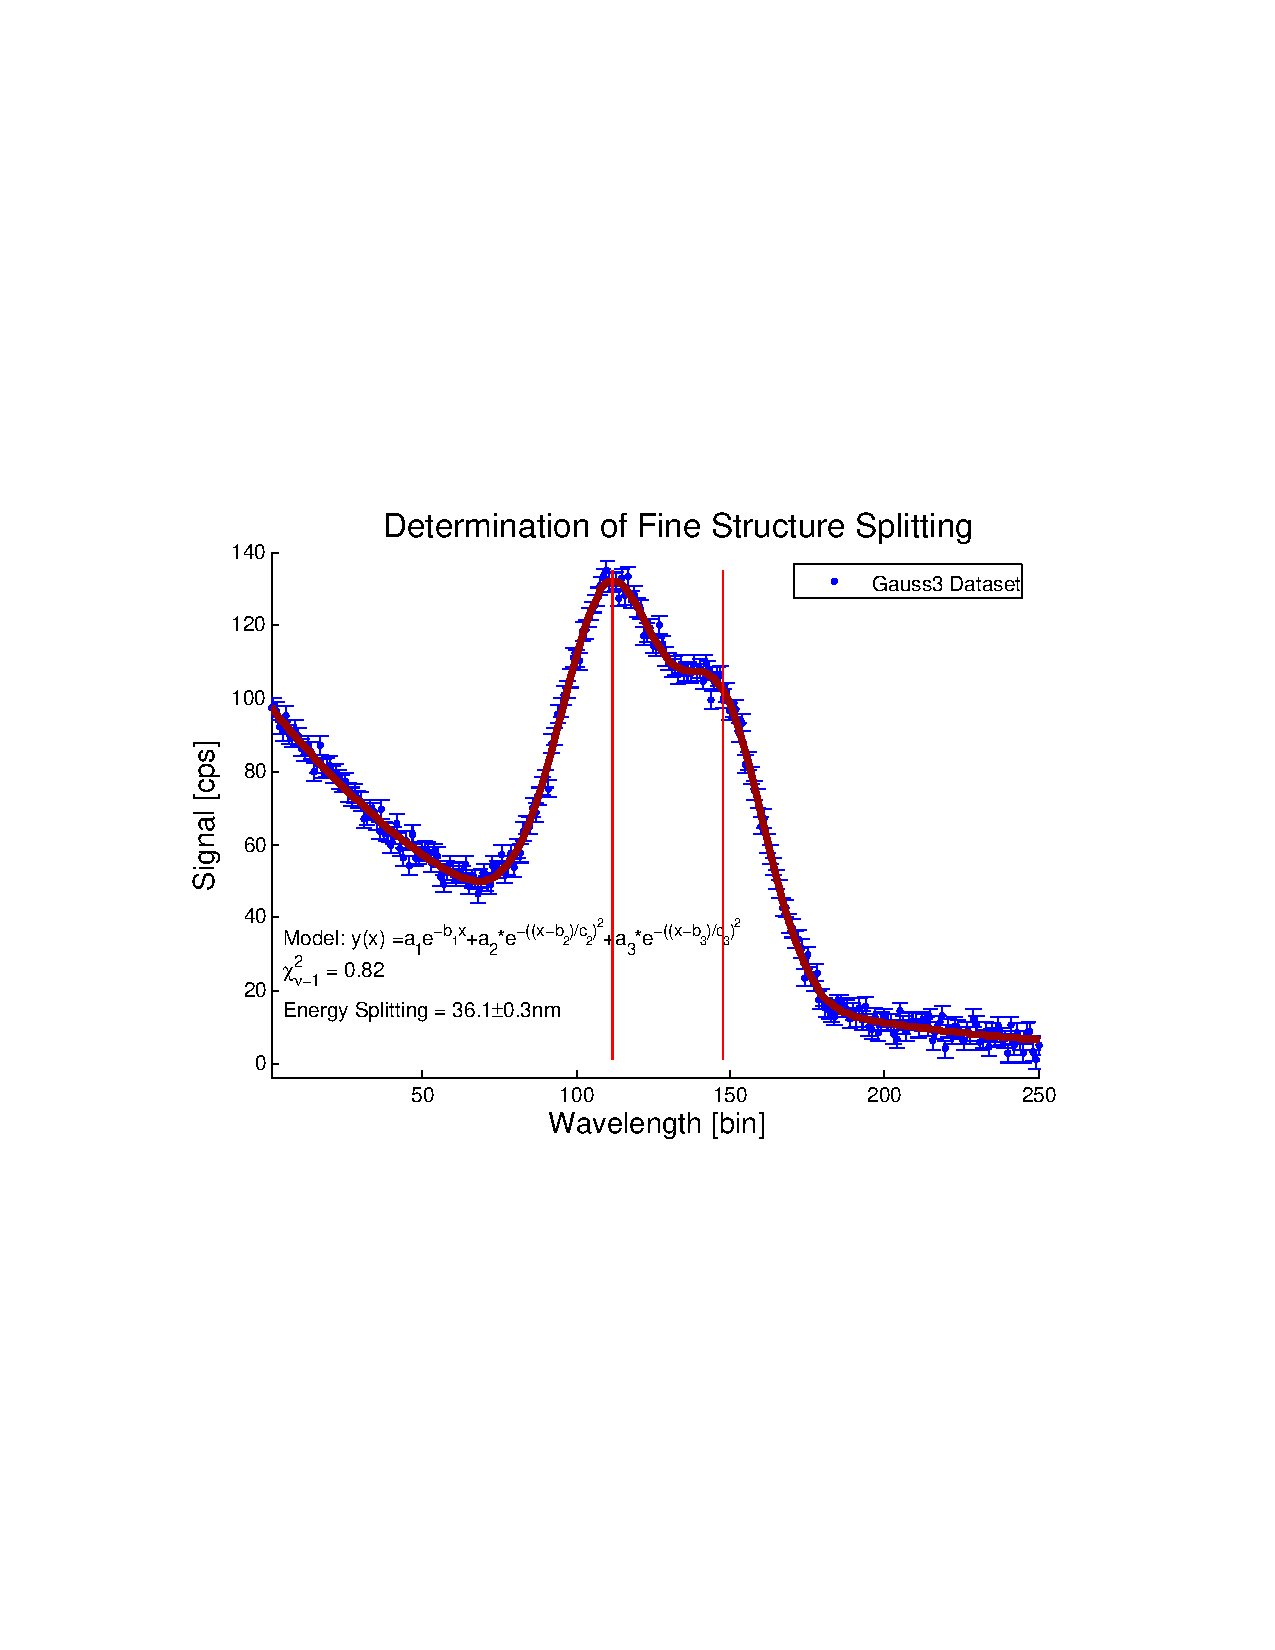
\includegraphics[width=9cm]{sample-fig2.pdf}
%\caption{Sample figure describing a set of data, fit procedures and
%results. Use the caption space to provide more details about the
%fitting procedure, results or implications if you do not have
%sufficient room in the main body of text. This figure was created
%using the Matlab script at
%\url{web.mit.edu/8.13/matlab/fittemplate07.m}}
%\label{fig:calibration}
%\end{figure}
%
%
%%\begin{figure*}[htb]
%%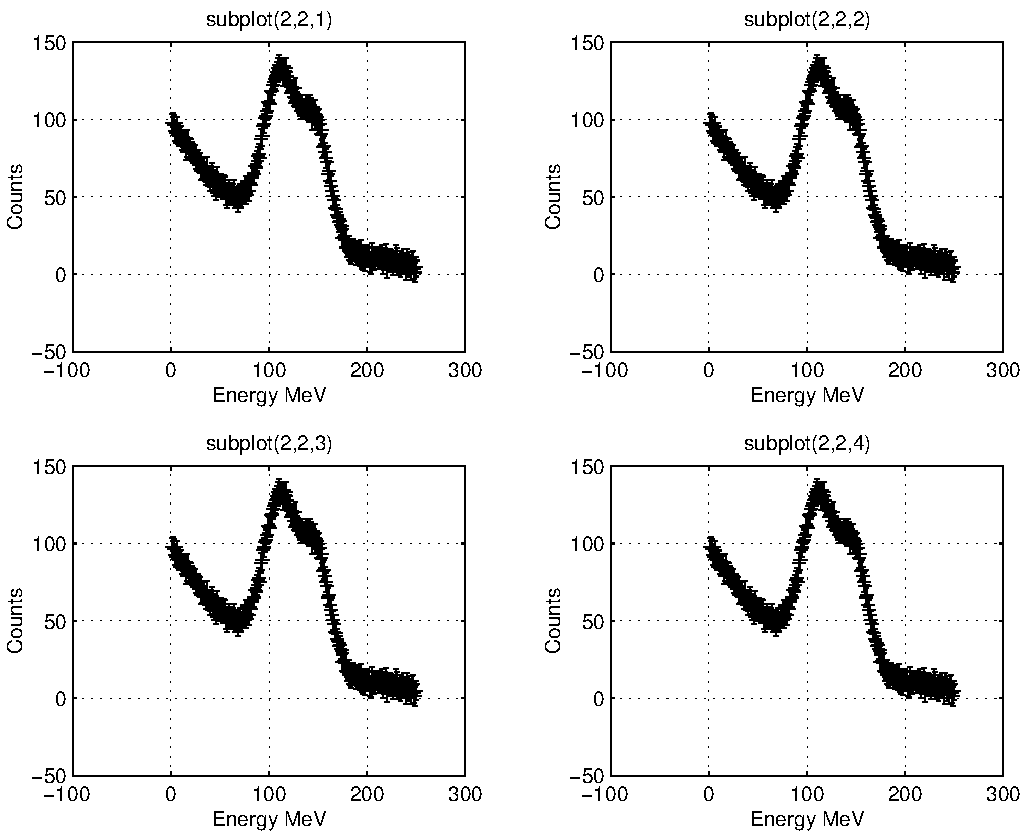
\includegraphics[angle=0,width=10cm]{sample-fig3}
%%\caption{Sample paneled figure created in Matlab using the
%%subplot(2,2,x) command where x is the element of the plot array into
%%which all subsequent commands such as plot(x,y) and xlabel('Volts'),
%%etc. get processed.  Use the caption space to provide more details
%%about the data, their acquisition or how they were processed if you do
%%not have sufficient room in the main body of text.  Figures can be
%%rotated using the angle command, see the TeX file for details.  If a
%%figure is to be placed after the main text use the ``figure*'' option
%%to make it extend over two columns, see the \LaTeX file for how this
%%was done.}
%%\label{fig:panel2x2}
%%end{figure*}
%
%\begin{figure}[htb]
%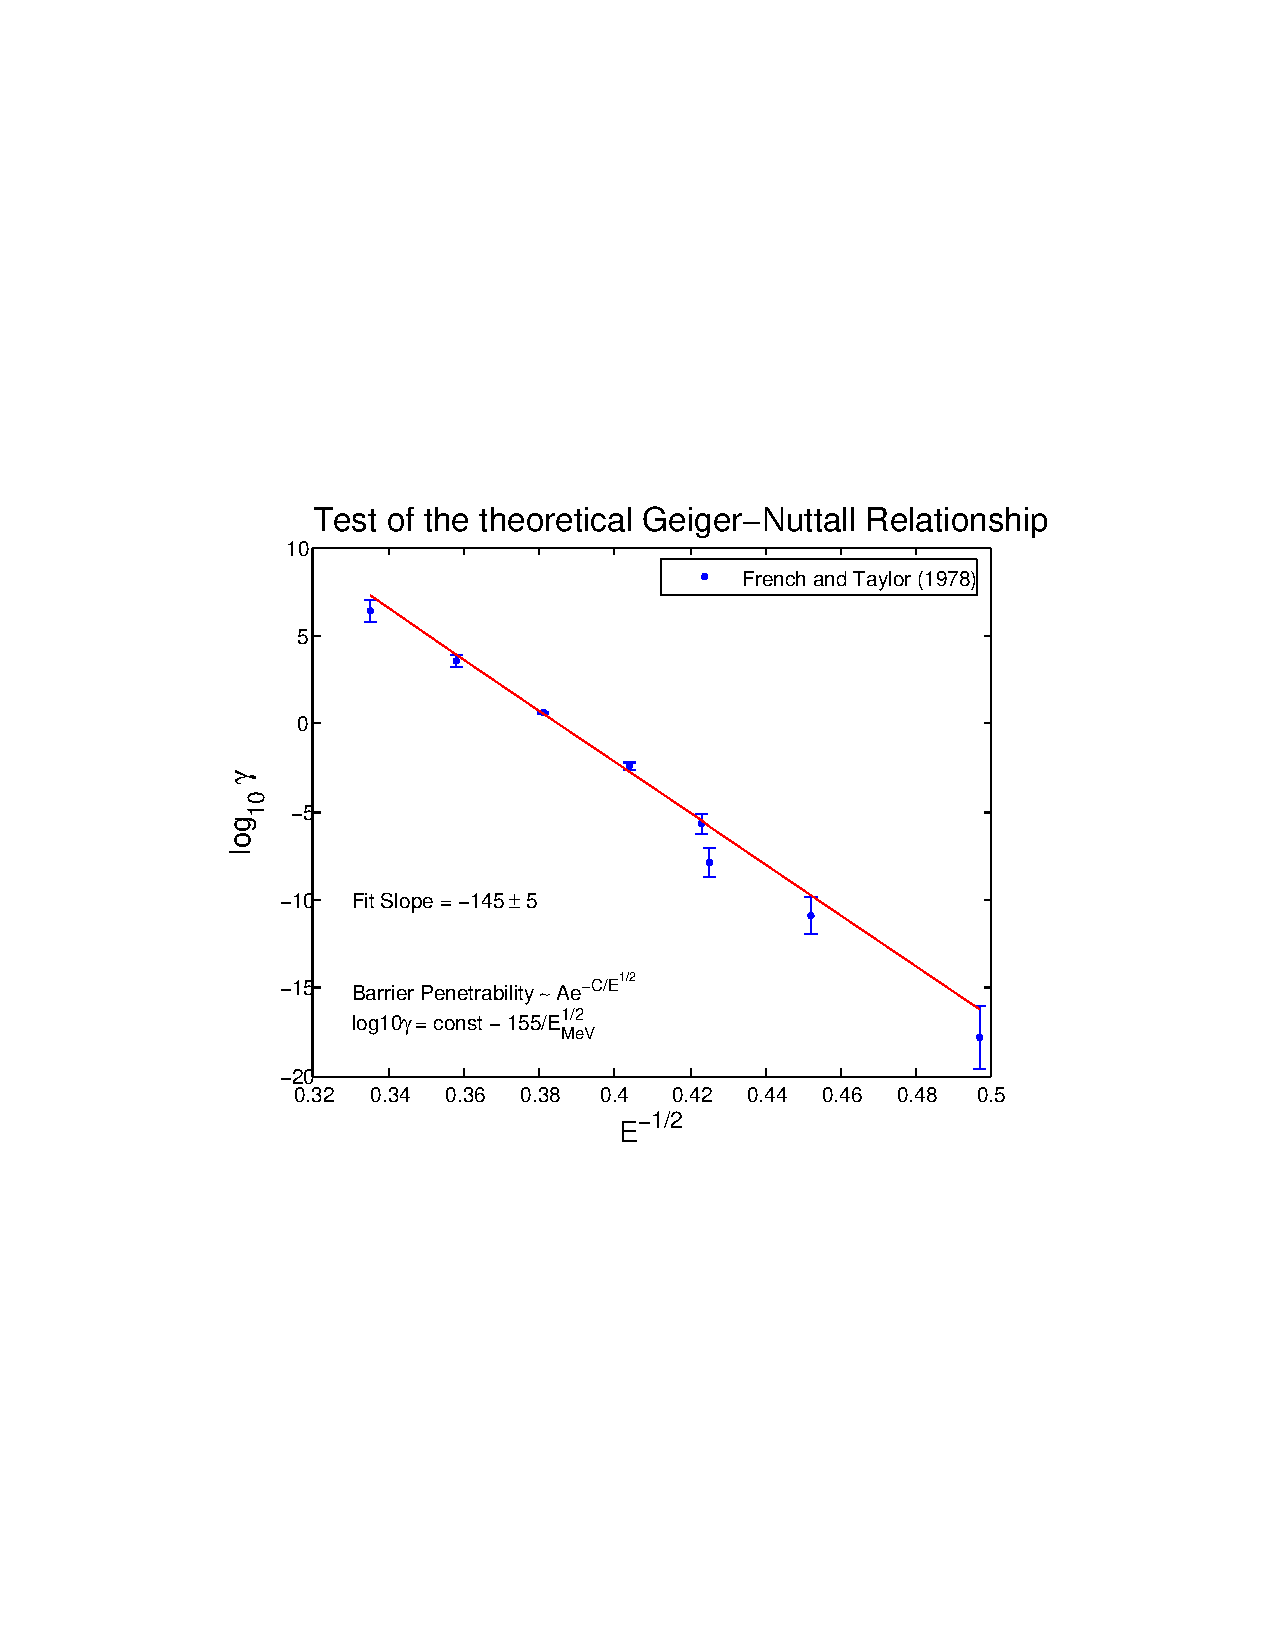
\includegraphics[width=9cm]{frenchtaylor.pdf}
%\caption{Sample figure showing overall physical relationship you set
%out to test.  This figure was created using the Matlab script at
%\url{web.mit.edu/8.13/matlab/fittemplate07.m}}
%\label{fig:frenchtaylor}
%\end{figure}
%
%Try to avoid the temptation to inundate the reader with too many
%graphics.  It is worth spending some time thinking of how best to
%present information rather than just creating graph after graph of
%uninformative data.  All figures and tables must be properly
%captioned.  Material and ideas drawn from the work of others must be
%properly cited, and a list of references should be included at the end
%of the text but before the graphics.
%
%\begin{table}[h]
%\caption{\label{tab:table1}A example table with footnotes.  Note
%that several entries share the same footnote. Always use a preceding
%zero in the data you record in tables.  Always display UNITS.
% Inspect the \LaTeX\ input for this table to see exactly how it is
%done.}
%\begin{ruledtabular}
%\begin{tabular}{cccccccc}
% &$r_c$ (\AA)&$r_0$ (\AA)&$\kappa r_0$&
% &$r_c$ (\AA) &$r_0$ (\AA)&$\kappa r_0$\\
%\hline
%Cu& 0.800 & 14.10 & 2.550 &Sn\footnotemark[1] & 0.680 & 1.870 & 3.700 \\
%Ag& 0.990 & 15.90 & 2.710 &Pb\footnotemark[1] & 0.450 & 1.930 & 3.760 \\
%Tl& 0.480 & 18.90 & 3.550 & & & & \\
%\end{tabular}
%\end{ruledtabular}
%\footnotetext[1]{Here's the first, from Ref.~\cite{bevington2003}.}
%\end{table}
%
%If circumstances in an experiment are such that you cannot get your
%own data (e.g. broken equipment, bad weather), {\bf you may use
%somebody else's data provided you acknowledge it}.
%
%
%%%%%%%%%%%%%%%%%%%%%%%%%%%%%%%%%%%%%%%%%%%%%%%%%%%%%%%%%%%%%%%%%%%%%%%%%%%%%%
\section{Conclusions}

Our results for $g=(9.781 \pm 0.017)\frac{m}{s^2}$ was very close to the accepted $g=9.80665 \frac{m}{s^2}$ with only a $0.262\%$ error, but our uncertainty was not enough to include the accepted value. This would indicate that either there was some additional source of error that we did not account for, or that we were imprecise in our measurements. As one possible improvement to this experiment, we would devise a consistent and reliable method to set the pendulum on the glass plates to reduce any additional drag. Another possible improvment would be reducing the skew of our measuring device, by manufacturing a alignment mechanism, or taking multiple periods at a given distance. I would say that we were mostly successful in our experiment, though there is room for improvement.
%
%And finally, conclusions.  Remember to report all your results with
%appropriate significant digits, units, and uncertainties, e.g. Q =
%(2.12 $\pm$ 0.06) disintegrations s$^{-1}$.  It is often very useful
%to express the quality of your result by measuring how many standard
%deviations it lies from other published values.
%
%It is worth mentioning here some thoughts on {\bf ethics and writing
%in Science}.
%
%When you read the report of a physics experiment in a reputable
%journal (e.g. Physical Review Letters) you can generally assume it
%represents an honest effort by the authors to describe exactly what
%they observed. You may doubt the interpretation or the theory they
%create to explain the results. But at least you trust that if you
%repeat the manipulations as described, you will get essentially the
%same experimental results.
%
%Nature is the ultimate enforcer of truth in science. If subsequent
%work proves a published measurement is wrong by substantially more
%than the estimated error limits, a reputation shrinks. If fraud is
%discovered, a career may be ruined. So most professional scientists
%are very careful about the records they maintain and the results and
%errors they publish.
%
%In keeping with the spirit of trust in science, Junior Lab instructors
%will assume that what you record in your lab book and report in your
%written and oral presentations is exactly what you have observed.
%
%{\bf Fabrication or falsification of data, using the results of
%another person's work without acknowledgement, or copying from {\em
%``living group files''} are intellectual crimes as serious as
%plagiarism, and possible causes for dismissal from USM.}
%
%{\bf The acknowledgement of other people's data also applies to the use
%of other people's rhetoric.} The appropriate way to incorporate an
%idea which you have learned from a textbook or other reference is to
%study the point until you understand it and then put the text aside
%and state the idea in your own words.
%
%One often sees, in a scientific journal, phrases such as ``Following
%Bevington and Melissinos \cite{bevington2003, melissinos1966} ...''
%This means that the author is following the ideas or logic of these
%authors and not their exact words.
%
%If you do choose to quote material, it is not sufficient just to
%include the original source among the list of references at the end of
%your paper. If a few sentences or more are imported from another
%source, that section should be
%
%\begin{quote}indented on both sides or enclosed in
%quotes, and attribution must be given immediately in the form of a
%reference note.\cite{melissinos1966}
%\end{quote}
%
%If you have any question at all about attribution of sources, please
%see you section instructor.
%
%Further information about how to avoid plagiarism is available
%online at \url{web.mit.edu/writing/Citation/plagiarism.html}.
%\section{Bibliography Remarks}
%Bibliographies are very important in Intermediate Physics Lab papers.  Beyond the
%requisite citation of source material, they provide evidence of your
%investigations beyond the narrow scope of the labguide, something
%explicitly required of all iLab students!  Good bibliographies
%are doubly important in the real world where they are very (often
%the most) important sources of information for researchers entering
%the field.  Bibliographic entries are made within a separate `.bib'
%file which gets attached during process of building a final PDF
%document.  See the file
%\url{web.mit.edu/8.13/www/Samplepaper/sample-paper.bib} for details
%on several types of bibliographic entries and their required and
%optional fields.
%
%%%%%%%%%%%%%%%%%%%%%%%%%%%%%%%%%%%%%%%%%%%%%%%%%%%%%%%%%%%%%%%%%%%%%%%%%%%%%%
%% Place all of the references you used to write this paper in a file
%% with the same name as following the \bibliography command
%%%%%%%%%%%%%%%%%%%%%%%%%%%%%%%%%%%%%%%%%%%%%%%%%%%%%%%%%%%%%%%%%%%%%%%%%%%%%%
%

\bibliographystyle{plainnat}
\bibliography{sample-paper.bib}
\nocite{*}
%
%
%%%%%%%%%%%%%%%%%%%%%%%%%%%%%%%%%%%%%%%%%%%%%%%%%%%%%%%%%%%%%%%%%%%%%%%%%%%%%%
\begin{acknowledgments} 
We wish to thank the University of Southern Maine for the opportunity to study and better ourselves. We wish to thank the Department of Paul Nakroshis (A.K.A. the Department of Physics) for giving us a community to encourage and support us. Finally we wish to thank Paul for guiding us in this Intermediate Laboratory Class, and passing along to us his passion in physics.
\end{acknowledgments}
%
%%%%%%%%%%%%%%%%%%%%%%%%%%%%%%%%%%%%%%%%%%%%%%%%%%%%%%%%%%%%%%%%%%%%%%%%%%%%%%
%\clearpage
%\appendix
%\section{\LaTeX~ Under Windows}
%For those students who would like to use a Windows platform, MiKTeX
%(pronounced \emph{mik-tech} is a freely available, implementation of
%TeX and related programs available from \url{www.miktex.org}. Note
%that MiKTeX itself runs from a command line prompt and is not terribly
%convenient.  We strongly recommend you simultaneously purchase and
%install a very nice TeX editor/shell called WinEdt, available from
%\url{www.winedt.com} for only \$30 for students. This interface is
%substantially easier than using `emacs' on Athena for writing and
%typesetting scientific papers and we encourage you to check it out.
%
%Once you've installed the above software, you will need to obtain
%the group of files listed in the next section and put them on your
%Windows machine in order to `rebuild' this document from scratch.
%
%
%If you wish to view postscript files under Windows, we
%suggest downloading and installing Ghostscript available from
%\url{www.cs.wisc.edu/~ghost}.
%
%\section{Useful  Utilities}
%{\bf Drawing Programs}
%
%Students should become proficient with a simple (vector based)
%computer drawing program such as {\bf Inkscape} or {\bf Asymptote}.
%Every written summary should include one or two simple schematics,
%based on their initial hand sketches from their lab notebooks.
%
%\section{Igor Pro and \LaTeX}
%Igor Pro is perhaps the most common tool used by iLab students
%for data analysis and representation.  Igor Pro figures can be saved
%directly into a `PDF' or `PNG' format obviating
%the need for any further format translation.
%
%
%% Surround figure environment with turnpage environment for landscape presentation
%\begin{turnpage}
%\begin{figure*}[htb]
%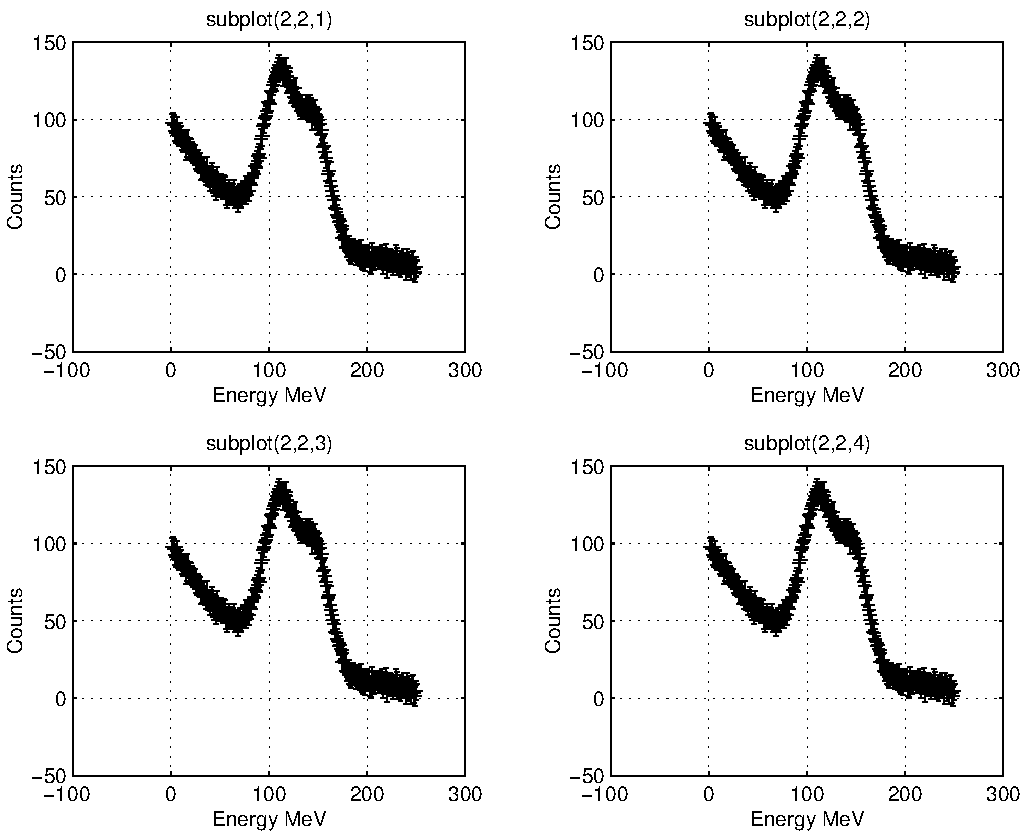
\includegraphics[width=20cm]{sample-fig3}
%\caption{For very large plots where important detail might be lost
%if too compressed, it can be convenient to use the `turnpage'
%environment for displaying in landscape mode. e.g. any experiment
%where a data set is acquired at several angular positions (21cm,
%e/m, Rutherford) or is time varying (Physics of Alpha Decay and
%Pulsed NMR.)  These full page graphics are usually best kept in
%appendices so as not to impede the flow of the paper.  Note that
%large tables can also be presented in this landscape environment if
%desired \label{fig:landscapegraphic}}
%\end{figure*}
%\end{turnpage}

% tables should appear as floats within the text
%
% Here is an example of the general form of a table:
% Fill in the caption in the braces of the \caption{} command. Put the label
% that you will use with \ref{} command in the braces of the \label{} command.
% Insert the column specifiers (l, r, c, d, etc.) in the empty braces of the
% \begin{tabular}{} command.
% The ruledtabular enviroment adds doubled rules to table and sets a
% reasonable default table settings.
% Use the table* environment to get a full-width table in two-column
% Add \usepackage{longtable} and the longtable (or longtable*}
% environment for nicely formatted long tables. Or use the the [H]
% placement option to break a long table (with less control than
% in longtable).
% \begin{table}%[H] add [H] placement to break table across pages
% \caption{\label{}}
% \begin{ruledtabular}
% \begin{tabular}{}
% Lines of table here ending with \\
% \end{tabular}
% \end{ruledtabular}
% \end{table}

% To convert program (e.g. C++ Fortran, Matlab, LaTeX) listings to a
% form easily includable in a LaTeX document
%
% type lgrind -s to see options
% lgrind -llatex -i sample-paper.tex > sampleinputtex
% creates a file sampleinput.tex which can then be included into this
% document simply by uncommenting the next line
%\lgrindfile{testinput.tex}

\end{document}
